\documentclass{article}
\usepackage[english]{babel}
\usepackage[utf8]{inputenc}
\usepackage{amsmath,amssymb}
\usepackage{parskip}
\usepackage{graphicx}
\usepackage{dsfont}
\usepackage{dsfont}
\usepackage{relsize}
\usepackage{array}
\newcommand{\bigsigma}{\makebox{\Huge\ensuremath{\sigma}}}
\newcommand{\bigpi}{\makebox{\Huge\ensuremath{\Pi}}}
\newcolumntype{C}[1]{>{\centering\let\newline\\\arraybackslash\hspace{0pt}}m{#1}}
\usepackage[top=2.5cm, left=3cm, right=3cm, bottom=4.0cm]{geometry}
\usepackage[table]{xcolor}
\usepackage[utf8]{inputenc}
\usepackage{textcomp}
\usepackage[utf8]{inputenc}
\usepackage{amsmath}
\usepackage{amssymb}
\usepackage{xcolor}
\usepackage{listings}
\usepackage{xstring}
\usepackage{graphicx}
\usepackage[export]{adjustbox}

\definecolor{dkgreen}{rgb}{0,0.6,0}
\definecolor{ltgray}{rgb}{0.5,0.5,0.5}

\makeatletter
\newif\ifcolname
\colnamefalse

\def\keywordcheck{%
\IfStrEq*{\the\lst@token}{select}{\global\colnametrue}{}%
\IfStrEq*{\the\lst@token}{where}{\global\colnametrue}{}%
\IfStrEq*{\the\lst@token}{from}{\global\colnamefalse}{}%
\color{blue}%
}
\def\setidcolor{%
\ifcolname\color{purple}\else\color{black}\fi%
}
\makeatother

\lstset{%
    backgroundcolor=\color{white},
    basicstyle=\footnotesize,
    breakatwhitespace=false,
    breaklines=true,
    captionpos=b,
    commentstyle=\color{dkgreen},
    deletekeywords={...},
    escapeinside={\%*}{*)},
    extendedchars=true,
    frame=single,
    keepspaces=true,
    language=SQL,
    otherkeywords={is},
    morekeywords={*,modify,MODIFY,...},
    keywordstyle=\keywordcheck,
    identifierstyle=\setidcolor,
    numbers=left,
    numbersep=15pt,
    numberstyle=\tiny,
    rulecolor=\color{ltgray},
    showspaces=false,
    showstringspaces=false, 
    showtabs=false,
    stepnumber=1,
    tabsize=4,
    title=\lstname
}

\newcommand{\tablespace}{\\[1.25mm]}
\newcommand\Tstrut{\rule{0pt}{2.6ex}}         % = `top' strut
\newcommand\tstrut{\rule{0pt}{2.0ex}}         % = `top' strut
\newcommand\Bstrut{\rule[-0.9ex]{0pt}{0pt}}   % = `bottom' strut
\title{Assignment-4 CS313}
\author{Shashank P \\ 200010048}
\date{\today}

\begin{document}
\maketitle




\section{Problem 1}
Create a user called universityDB0048.
\begin{lstlisting}[language=sql]
  create user 'universityDB0048'@'localhost' identified by 'MyPassword@123';
  grant all privileges on university.* to 'universityDB0048'@'localhost';
  /* Logout and login as user universityDB0048 */
\end{lstlisting}
\begin{figure}[!ht]
  \begin{center}
  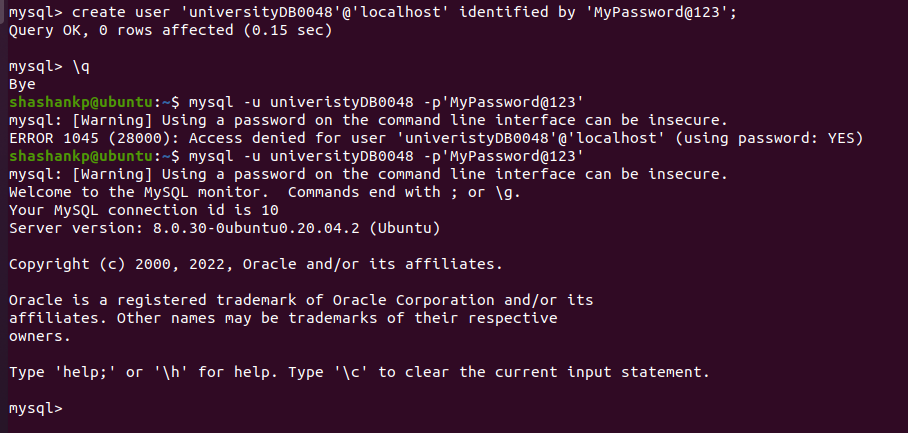
\includegraphics[scale=0.8]{Q1.png}
  \caption{Creation of User and adding previleges}
  \end{center}
\end{figure}

\newpage
\section{Problem 2}
Create a database called university.
\begin{lstlisting}[language=sql]
  create database university;
\end{lstlisting}
\begin{figure}[!ht]
  \begin{center}
  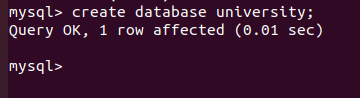
\includegraphics[scale=0.8]{Q2.png}
  \caption{Create Database}
  \end{center}
\end{figure}

\newpage
\section{Problem 3}
Use the database named university.
\begin{lstlisting}[language=sql]
  use university;
\end{lstlisting}
\begin{figure}[!ht]
  \begin{center}
  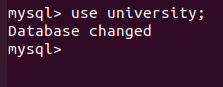
\includegraphics[scale=0.8]{Q3.png}
  \caption{Use Database}
  \end{center}
\end{figure}

\newpage
\section{Problem 4}
Create the tables in the university database using DDL.sql file.
\begin{lstlisting}[language=sql]
  source DDL.sql;
\end{lstlisting}
\begin{figure}[!ht]
  \begin{center}
  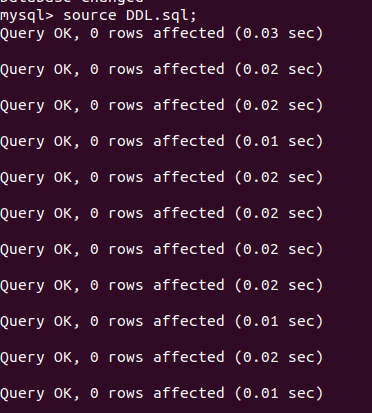
\includegraphics[scale=0.8]{Q4_2.png}
  \caption{Create Output}
  \end{center}
\end{figure}
\begin{figure}[!ht]
  \begin{center}
  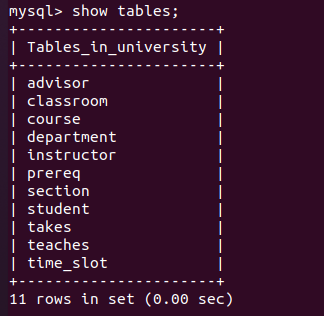
\includegraphics[scale=0.8]{Q4.png}
  \caption{Create Tables}
  \end{center}
\end{figure}

\newpage
\section{Problem 5}
Load the data into tables using InsertValues.sql.
\begin{lstlisting}[language=sql]
  source InsertValues.sql;
\end{lstlisting}
\begin{figure}[!ht]
  \begin{center}
  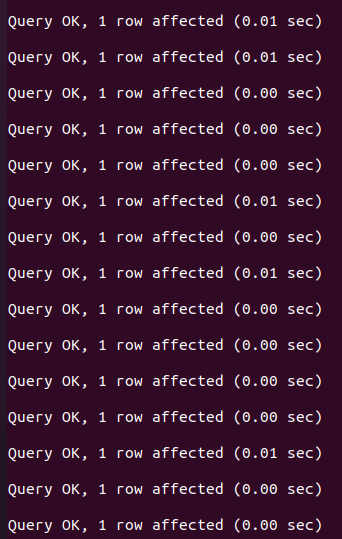
\includegraphics[scale=0.6]{Q5_2.png}
  \caption{Insert QUery Output}
  \end{center}
\end{figure}
\begin{figure}[!ht]
  \begin{center}
  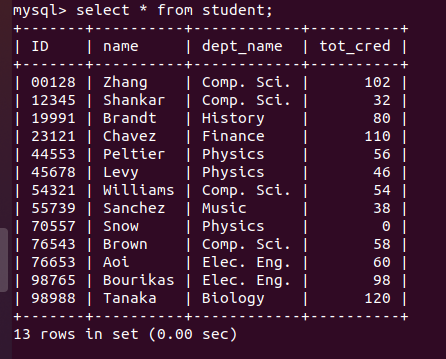
\includegraphics[scale=0.6]{Q5.png}
  \caption{Insert into Tables (Example: student table)}
  \end{center}
\end{figure}


\newpage
\section{Problem 6}
Get the details of all the tables using informatio\_schema.
\begin{lstlisting}[language=sql]
  select table_name, column_name, data_type from information_schema.columns;
\end{lstlisting}
\begin{figure}[!ht]
  \begin{center}
  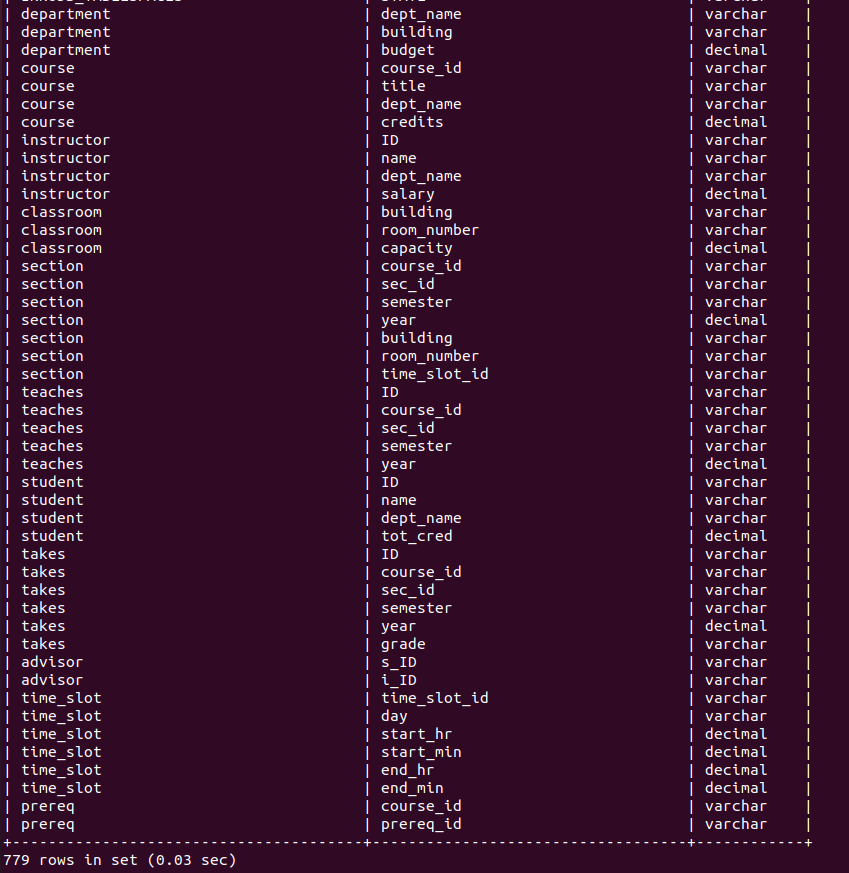
\includegraphics[scale=0.7]{Q6.png}
  \caption{Schema Information for each table}
  \end{center}
\end{figure}

\newpage

\section{Problem 7}
\subsection{Login}
Login to the user which you have created in Question number 1.
\begin{figure}[!ht]
  \begin{center}
  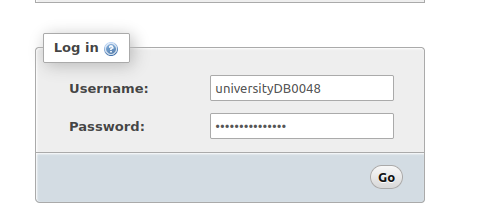
\includegraphics[scale=1]{Q7_1.png}
  \caption{Logging into phpmyadmin}
  \end{center}
\end{figure}

\newpage
\subsection{University Database}
Use database University.
\begin{figure}[!ht]
  \begin{center}
  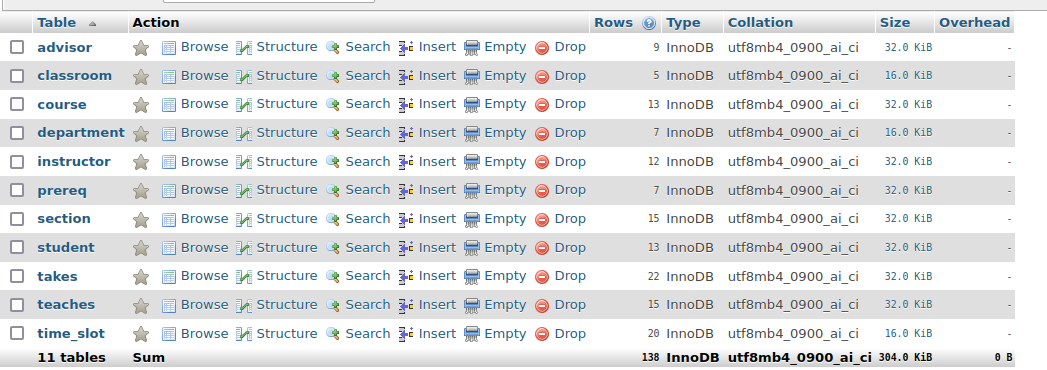
\includegraphics[scale=0.7]{Q7_2.png}
  \caption{Using university database}
  \end{center}
\end{figure}

\newpage
\subsection{Select and Insert Queries}
Performed select and insert queries on each table.
\begin{lstlisting}[language=sql]
  insert into department values('My New Department', 'Watson', 200000);
  select * from department where budget between 50000 and 210000;

  insert into course values('NN-101', 'A New Course', 'History', 5);
  select max(credits) from course;

  insert into instructor values('12345', 'A New Instructor', 'Comp. Sci.', 50000);
  select ID, name from instructor where dept_name in ('Comp. Sci.', "Physics");

  insert into section values('CS-101', '3', 'Summer', 2019, 'Watson', '100', 'A');
  select * from section where course_id='CS-101' order by time_slot_id asc;

  insert into teaches values('45565', 'CS-101', '1', 'Fall', 2009);
  select max(year), min(year) from teaches where ID='45565';

  insert into student values('99999', 'New Name', 'Comp. Sci.', 250);
  select ID, name from student where tot_cred in (select max(tot_cred) from student);

  insert into takes values('44553', 'CS-347', '1', 'Fall', 2009, 'A-');
  select * from takes where ID=='44553';

  insert into advisor values('19991', '22222');
  select * from advisor where i_ID='22222';

  insert into time_slot values('NEW', 'R', 13, 31, 14, 45);
  select * from time_slot where day='R';

  insert into prereq values('PHY-101', 'BIO-101');
  select * from prereq where prereq_id='BIO-101';
\end{lstlisting}
\begin{figure}[!ht]
  \begin{center}
  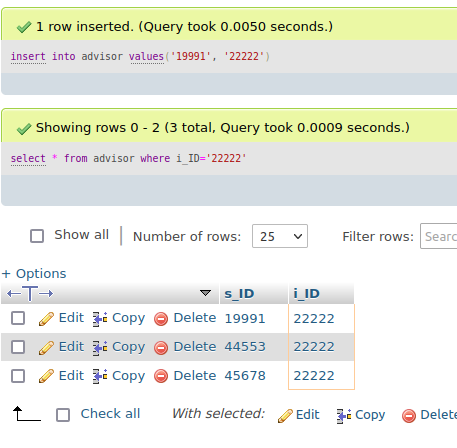
\includegraphics[scale=0.7]{Q7_3.png}
  \caption{Select and Insert (Ex: advisor table)}
  \end{center}
\end{figure}


\newpage

\section{Problem 8}
\subsection{Question 1}
Instructors from CSE department teaching Civil courses. Since there was no such data I have inserted
an instructor and a course that satisfy these conditions.
\begin{lstlisting}[language=sql]
  select distinct(course.course_id), course.title, instructor.ID, instructor.name
  from (instructor natural join teaches), course
  where course.course_id=teaches.course_id 
    and instructor.dept_name='Comp. Sci.'
    and teaches.year=2009 
      and course.dept_name='Civil'
  order by instructor.name ASC;
\end{lstlisting}
\begin{figure}[!ht]
  \begin{center}
  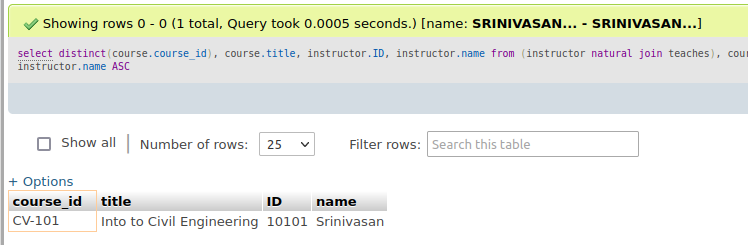
\includegraphics[scale=1]{Q8_1.png}
  \caption{Question 1}
  \end{center}
\end{figure}

\newpage

\subsection{Question 2}
Insert a new course and its pre-requisite.
\begin{lstlisting}[language=sql]
  insert into course values('CS-303', 'DBIS', 'Comp. Sci.', 6),
  ('CS-333', 'New Course', 'Comp. Sci.', 3);
  insert into prereq values('CS-333', 'CS-303');
  select * from prereq;
\end{lstlisting}
\begin{figure}[!ht]
  \begin{center}
  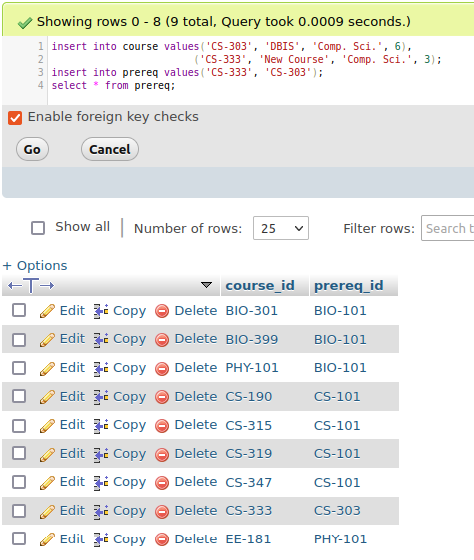
\includegraphics[scale=1]{Q8_2.png}
  \caption{Question 2}
  \end{center}
\end{figure}

\newpage

\subsection{Question 3}
Increment salaries of instructors whose department budget is greater than 90000.
\begin{lstlisting}[language=sql]
  update instructor
  set salary = salary*1.1
  where dept_name in (select department.dept_name 
                      from department 
                      where departmenet.budget>90000);
\end{lstlisting}
\begin{figure}[!ht]
  \begin{center}
  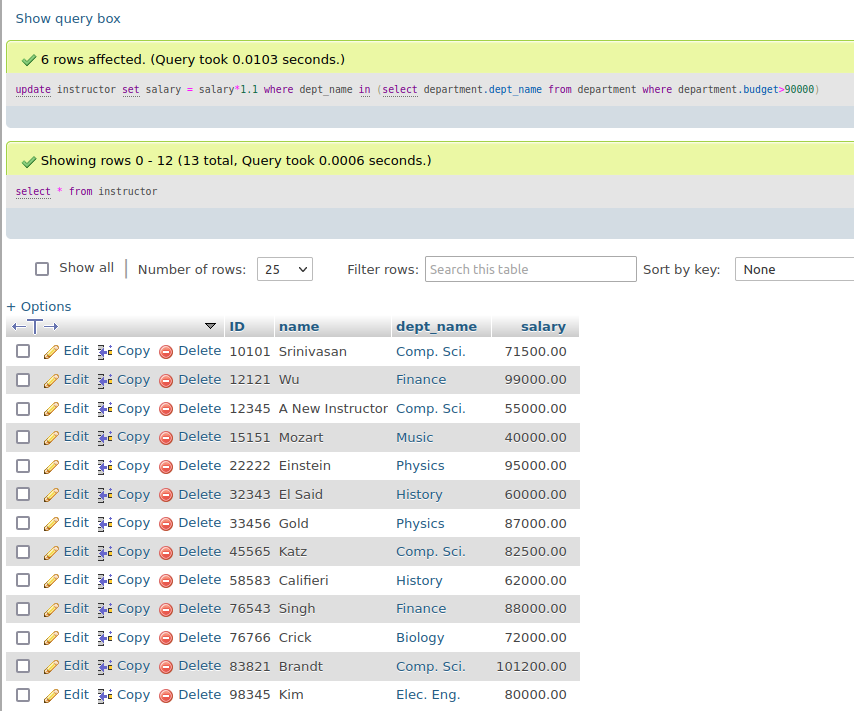
\includegraphics[scale=0.7]{Q8_3.png}
  \caption{Question 3}
  \end{center}
\end{figure}

\newpage

\subsection{Question 4}
Get Courses taken by some minimum number of students based on semester and year. Since no such
data existed I have modified the values of the query keeping the essence of the question same.
\begin{lstlisting}[language=sql]
  select count(ID), course_id
  from takes natural join course
  where course.dept_name="Comp. Sci."
      and takes.year=2009
      and takes.semester="Fall"
  group by course_id
  having count(ID)>2
  order by course_id ASC;
\end{lstlisting}
\begin{figure}[!ht]
  \begin{center}
  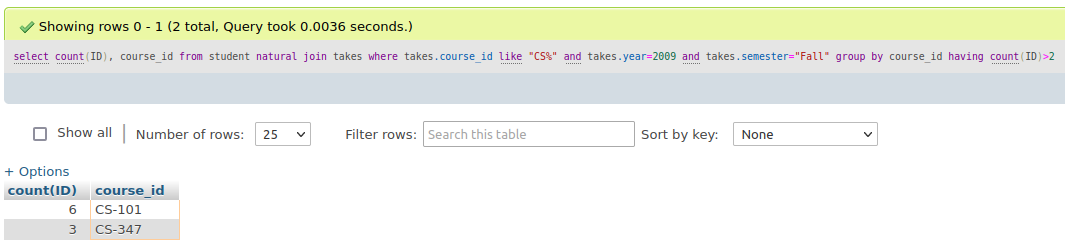
\includegraphics[scale=0.7]{Q8_4.png}
  \caption{Question 4}
  \end{center}
\end{figure}

\end{document}
